%% !TEX root = ../Thesis.tex
%% !TEX output_directory
\documentclass[11pt,a4paper,english,greek,twoside]{../Thesis}
\begin{document}
\chapter{Εισαγωγή}
\section{Σημασία Μελέτης Εγκεφάλου και Βιοηλεκτρικών Σημάτων}
\label{sec:importance}
Ο ανθρώπινος εγκέφαλος, είναι ίσως η πιο περίπλοκη δομή που γνωρίζουμε. Περίπου 86 δισεκατομμύρια νευρώνες \cite{Herculano-Houzel2009-vm} αλληλεπιδρούν δυναμικά μεταξύ τους δημιουργώντας τρισεκατομμύρια συνάψεις. Οι γνωσιακές επιστήμες συνδυάζοντας γνώση από τους τομείς της ψυχολογίας της νευρολογίας καθώς και με την βοήθεια υπολογιστικών μεθόδων, προσπαθούν να προσεγγίσουν την περίπλοκη λειτουργία του εγκεφάλου. Ένας τρόπος να εξερευνηθούν οι λειτουργίες του εγκεφάλου είναι μέσω της αλληλεπίδρασης του με το εξωτερικό περιβάλλον, υλοποιώντας, συσκευές οι οποίες ανιχνεύουν την εγκεφαλική δραστηριότητα και την μεταφράζουν σε μηνύματα ή εντολές. Μέσω αυτών των συσκευών, δίνεται η δυνατότητα να ληφθούν συμπεράσματα για την λειτουργία συγκεκριμένων περιοχών του εγκεφάλου, χωρίς απαραίτητα να γνωρίζουμε λεπτομέρειες όσον αφορά τους νευρώνες και το πως αλληλεπιδρούν. Αυτές οι συσκευές ονομάζονται Διεπαφές Εγκεφάλου Υπολογιστή (Brain Computer Interfaces - BCI) και τα τελευταία χρόνια παρατηρείται σημαντική αύξηση στις ερευνητικές ομάδες που κάνουν δημοσιεύσεις σε αυτόν τον τομέα \cite{nicolas2012brain}. Εκτός όμως από την χρήση τους για την ερμηνεία της εγκεφαλικής δραστηριότητας, σημαντική είναι η συνεισφορά τους σε άτομα με αναπηρίες, στους οποίους προσφέρει μια δίοδο επικοινωνίας με το περιβάλλον, η οποία υπό άλλες συνθήκες θα ήταν αδύνατο να επιτευχθεί. Τα παραδείγματα είναι πάρα πολλά, μέσω των BCIs, άτομα με αναπηρία είναι ικανά να μετακινήσουν προσθετικά μέλη \cite{Bandara2018-bf}\cite{Muller-Putz2008-gd}\cite{Agashe2015-kx}, να χρησιμοποιήσουν μηχανές συλλαβισμού (spellers)\cite{Bin2011-eh}\cite{Nakanishi2018-sc}, να πλοηγηθούν στο Internet \cite{Mugler2010-rs}, ή να κατευθύνουν το αναπηρικό τους αμαξίδιο \cite{Li2013-qt}\cite{Cao2014-wz}.  
\begin{figure}[H]
    \centering     %%% not \center
    \subfigure[]{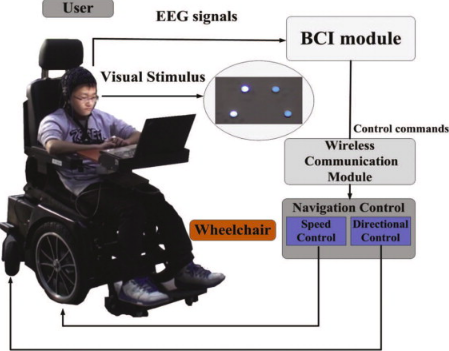
\includegraphics[scale=0.4]{{{ImagesSSVEP/wheelchair}.png}}} % \cite{Cao2014-wz}
    \subfigure[]{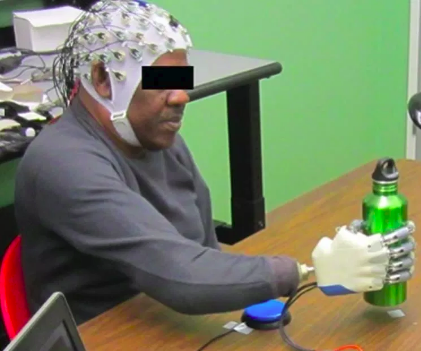
\includegraphics[scale=0.4]{{{ImagesSSVEP/prosthetic}.png}}} %Agashe2015-kx
    \caption{a) Παράδειγμα αναπηρικού αμαξιδίου με ενσωματωμένο σύστημα BCI. Εικόνα από \cite{Cao2014-wz} b) Διάταξη BCI συστήματος, στο οποίο η σκεψη της κίνησης του χεριού, μεταφράζεται σε πραγματική κίνηση του προσθετικού μέλους. Εικόνα από \cite{Agashe2015-kx}}
    \label{fig:bci_examples}
\end{figure}
\par Ωστόσο, το πλήθος των ανθρώπων που κάνουν χρήση τέτοιων διεπαφών είναι ελάχιστο, και αυτό επειδή ακόμα η έρευνα σε αυτόν τον τομέα παραμένει μέσα στα εργαστήρια. Υπάρχουν κάποιοι βασικοί λόγοι που συμβαίνει αυτό. Ένας από αυτούς είναι η χρονοβόρα προετοιμασία που απαιτείται για την χρήση του εγκεφαλογράφου και την εκπαίδευση του ατόμου να τον χρησιμοποιεί \cite{blankertz2010berlin}. Επιπλέον η χρήση τέτοιον διεπαφών σε μη ελεγχόμενα εργαστηριακά περιβάλλοντα, εισάγει εμπόδια στην διαδικασία, όπως ανεπιθύμητες παρεμβολές στα σήματα και λάθη των χρηστών κατά τη διάρκεια της χρήσης. Τέλος, οι εγκεφαλογράφοι που χρησιμοποιούνται στην έρευνα και επιτυγχάνουν state-of-the-art επιδόσεις, προορίζονται για ιατρικές εφαρμογές, και το κόστος τους είναι υπέρογκο για να αποκτηθούν ατομικά από έναν χρήστη. Κρίνεται συνεπώς απαραίτητη, αρχικά η κατασκευή οικονομικότερων εγκεφαλογράφων, που στοχεύουν σε χρήστες εκτός των εργαστηρίων, και κατά δεύτερον, η ανάπτυξη υπολογιστικών μεθόδων που θα καταστήσουν την επίδοση αυτών των εγκεφαλογράφων συγκρίσιμη με ακριβότερα μοντέλα. 


\section{Σκοπός και Συνεισφορά της Διπλωματικής Εργασίας}
Στόχος αυτής της διπλωματικής εργασίας είναι η υλοποίηση μιας διεπαφής εγκεφάλου υπολογιστή βασιζόμενη σε μια κατηγορία οπτικών προκλητών δυναμικών που ονομάζονται Steady State Visual Evoked Potentials. Σε αντίθεση όμως με την πλειοψηφία της έρευνας σε αυτόν τον τομέα, όπου γίνεται χρήση ακριβών εγκεφαλογράφων κατασκευασμένων για ιατρική χρήση, σε αυτή την εργασία γίνεται χρήση ενός low-budget εγκεφαλογράφου (Emotiv Epoc), πράγμα που αποτελεί και την βασική πρόκληση της εργασίας. Η όλη πειραματική διαδικασία, το hardware για την δημιουργία των οπτικών ερεθισμάτων, η γραφική διεπαφή για την παρακολούθηση των εγκεφαλικών σημάτων σε πραγματικό χρόνο, καθώς και ένα σύνολο συναρτήσεων για την επεξεργασία των εγκεφαλικών σημάτων στην προγραμματιστική γλώσσα Python, σχεδιάστηκαν και υλοποιήθηκαν εξολοκλήρου στα πλαίσια της εργασίας. Επιπλέον, δημιουργήσαμε ένα dataset με όλες τις καταγραφές εγκεφαλογραφήματος που έλαβαν μέρος κατά την διάρκεια της εργασίας, ταξινομημένες ανά άτομο, έτσι ώστε όλα αυτά μαζί να αποτελέσουν εφαλτήριο για περαιτέρω έρευνα πάνω στο συγκεκριμένο θέμα. Όσον αφορά τους αλγορίθμους που χρησιμοποιήθηκαν για την εξαγωγή πληροφορίας από τα εγκεφαλικά σήματα, δοκιμάστηκαν διάφορες μέθοδοι που χρησιμοποιούνται κατά κόρον στην βιβλιογραφία, και είδαμε πως στην offline επεξεργασία των σημάτων, η απόδοση του συστήματος συγκρίνεται με τις state-of-the-art επιδόσεις για low-budget εγκεφαλογράφους και άλλων παρόμοιων διατάξεων. Τέλος υλοποιήσαμε την online εκδοχή της διεπαφής, με δυνατότητα πέρα από την αναγνώριση των SSVEP σημάτων, την ανίχνευση δύο ακόμα εντολών-καταστάσεων: κλείσιμο ματιών και κατάσταση αδράνειας στην οποία ο χρήστης δεν επιθυμεί να στείλει κάποια εντολή, και παρουσιάσαμε τα αποτελέσματα και τα συμπεράσματα για το κατά πόσο η μεθοδολογία μας και ο εγκεφαλογράφος Epoc, ικανοποίησαν τις προσδοκίες.

\section{Διάρθρωση Διπλωματικής Εργασίας}
\par Η εργασία ακολουθεί την εξής πορεία:
\begin{itemize}
	\item Στο κεφάλαιο 2 παρουσιάζεται το θεωρητικό υπόβαθρο γύρω από την εγκεφαλογραφία, τις διεπαφές εγκεφάλου - υπολογιστή, καθώς και τα πιο γνωστά εγκεφαλικά σήματα.
	\item Στο κεφάλαιο 3 γίνεται μια ανασκόπηση των υπολογιστικών μεθόδων που για την προεπεξεργασία των σημάτων, την εξαγωγή των χαρακτηριστικών, καθώς και στις μεθόδους μηχανικής μάθησης που θα χρησιμοποιηθούν
	\item Στο κεφάλαιο 4 γίνεται μια σύντομη ανασκόπηση των state of the art SSVEP BCI, καθώς και των δημοσιεύσεων υλοποίησαν διεπαφές βασισμένες στον συνδυασμό Epoc-SSVEP
	\item Στο κεφάλαιο 5 παρουσιάζεται η διεπαφή που υλοποιήθηκε. Αρχικά γίνεται μια αναλυτική περιγραφή του εγκεφαλογράφου Emotiv Epoc, καθώς και του υλικού και λογισμικού, που κατασκευάστηκε για την δημιουργία των οπτικών ερεθισμάτων. Έπειτα περιγράφονται ακριβώς οι διαδικασίες της offline ανάλυσης των σημάτων, οπού έγινε πειραματισμός με διάφορες μεθόδους, ενώ στην πορεία παρουσιάζεται και η υλοποίηση της online διεπαφής.
	\item Στο κεφάλαιο 6 παραθέτονται τα αποτελέσματα για κάθε χρήστη, τόσο στην offline και online διεπαφλη , 
	\item Στο κεφάλαιο 7 κλείνουμε αυτή την εργασία κάνοντας την σύνοψη, και προτείνοντας μελλοντικές ερευνητικές κατευθύνσεις. 
\end{itemize}

\end{document}
